% =====================================================================
%  Research Statement -- Computer Science (generic version)
%  Lead theme: trustworthy / certified scientific machine learning
%  Davood Damircheli, Department of Mathematics, Louisiana State University
%  Compile: pdflatex (twice)
%
%  Lines marked  %CHECK  contain claims that should be confirmed before
%  submission (authorship of in-preparation drafts, final numbers, etc.).
%  Labels in [ ] match the applied-math statement and the CV; M3/M4 are
%  new labels for drafts not yet on the CV.
% =====================================================================
\documentclass[11pt]{article}
\usepackage[letterpaper,hmargin=1in,vmargin=0.85in]{geometry}
\usepackage[T1]{fontenc}
\usepackage{mathpazo}
\usepackage[scaled=0.95]{helvet}
\usepackage{microtype}
\usepackage{amsmath,amssymb}
\usepackage{xcolor}
\usepackage{enumitem}
\usepackage{titlesec}
\usepackage{tikz}
\usetikzlibrary{positioning,arrows.meta,shapes.misc}
\usepackage[hidelinks]{hyperref}

\definecolor{accent}{RGB}{25,70,125}
\definecolor{soft}{RGB}{235,241,248}
\definecolor{okgreen}{RGB}{30,120,70}
\definecolor{badred}{RGB}{170,40,40}

\titleformat{\section}{\normalfont\large\bfseries\color{accent}}{\thesection.}{0.5em}{}
\titlespacing*{\section}{0pt}{9pt}{3pt}
\titleformat{\paragraph}[runin]{\normalfont\bfseries}{}{0pt}{}[.]
\titlespacing*{\paragraph}{0pt}{4pt}{0.6em}
\setlist{nosep,leftmargin=1.3em,topsep=2pt}
\setlength{\parskip}{3pt}
\setlength{\parindent}{0pt}

\renewcommand{\ttdefault}{pcr}
\newcommand{\rc}[1]{\textcolor{accent}{[#1]}}

\begin{document}

% ------------------------------------------------------------- header
\begin{center}
{\LARGE\bfseries Research Statement}\\[3pt]
{\large Davood Damircheli}\\[1pt]
{\small Department of Mathematics, Louisiana State University\\
\href{mailto:ddamircheli@lsu.edu}{ddamircheli@lsu.edu} \;$\cdot$\;
\href{https://davooddamircheli.github.io}{\nolinkurl{davooddamircheli.github.io}} \;$\cdot$\;
\href{https://github.com/DavoodDamircheli}{\nolinkurl{github.com/DavoodDamircheli}}}
\end{center}
\vspace{-4pt}

% ------------------------------------------------------------- overview
\section*{Overview}

Machine-learned models are quickly replacing numerical solvers in science and
engineering: neural networks and reduced-order surrogates now price financial
contracts, predict fracture, and stand in for expensive simulations inside
design loops. They are fast, but they fail \emph{silently}. A surrogate gives
no warning when a query falls outside its training distribution, when a
physical constraint is violated, or when training has converged to the wrong
answer. My research asks a question that is at once computational and
mathematical: \emph{how can we certify, for a given input and at run time,
that a computed or learned answer is correct?}

I answer it with three kinds of tools, which I develop together:
\begin{enumerate}[label=(\roman*),leftmargin=2.2em]
\item \textbf{Verification of learned solvers}: computable, mathematically
      guaranteed error bounds---evaluated with validated (interval) arithmetic
      where needed---that accept, correct, or reject the output of a neural or
      reduced model query by query;
\item \textbf{Structure-exploiting algorithms}: discretizations and solvers
      that keep the property responsible for stability and speed (Toeplitz
      structure, coercivity, algebraic cancellation, minimum residual), so that
      the reference solvers behind a certificate are fast and provably convergent;
\item \textbf{Scalable simulation and open software}: parallel 3D simulation
      of fracture in granular media on up to 1{,}600 cores, and a correctness
      theory for the event-driven code that runs it.
\end{enumerate}
My training spans both sides of this question: two Ph.D.s from Mississippi
State (computational engineering and applied mathematics), and postdoctoral
work in Robert Lipton's group at LSU on two DoD MURI awards projects in
computational mechanics. %CHECK: "MURI" wording if you want to use it here
The applications that drive my work---computational finance and fracture
mechanics---are ones where a wrong number has real cost.

\begin{center}
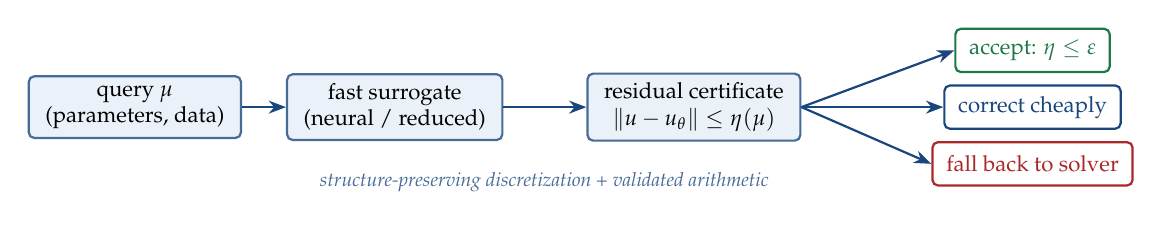
\begin{tikzpicture}[
  font=\footnotesize,
  box/.style={rectangle, rounded corners=2pt, draw=accent!80, fill=soft, thick, minimum height=7mm, inner xsep=6pt, align=center},
  out/.style={rectangle, rounded corners=2pt, draw=#1, fill=white, thick, minimum height=5.5mm, inner xsep=5pt, align=center, text=#1},
  arr/.style={-{Stealth[length=2.2mm]}, accent, thick}]
  \node[box] (q) at (0,0) {query $\mu$\\(parameters, data)};
  \node[box] (s) at (3.3,0) {fast surrogate\\(neural / reduced)};
  \node[box] (c) at (7.1,0) {residual certificate\\$\|u-u_\theta\|\le\eta(\mu)$};
  \node[out=okgreen] (a) at (11.4,0.72) {accept: $\eta\le\varepsilon$};
  \node[out=accent] (k) at (11.4,0) {correct cheaply};
  \node[out=badred] (r) at (11.4,-0.72) {fall back to solver};
  \draw[arr] (q) -- (s);
  \draw[arr] (s) -- (c);
  \draw[arr] (c.east) -- (a.west);
  \draw[arr] (c.east) -- (k.west);
  \draw[arr] (c.east) -- (r.west);
  \node[font=\scriptsize\itshape, text=accent!80] at (5.2,-0.95)
     {structure-preserving discretization + validated arithmetic};
\end{tikzpicture}
\end{center}
\vspace{-8pt}

% ------------------------------------------------------------- theme 1
\section{Certifying machine-learned solvers}

\paragraph{Guaranteed error bounds for neural networks on free-boundary problems}
Constrained problems---obstacles, free boundaries, contact---are where neural
PDE solvers fail most quietly, because a network can look accurate while
violating the constraint. In \rc{P1} I proved and implemented
guaranteed error bounds for neural approximations of parabolic obstacle
problems (variational inequalities that include American option pricing and
Stefan-type melting). The key idea is to certify not the network $v$ but its
\emph{feasible projection} $\hat v=\max\{v,g\}$; this removes every
constraint-violation term and every hard-to-estimate stability constant from
the bound. All integrals in the certificate are evaluated with outward-rounded
Taylor-model enclosures (interval arithmetic, Arb library), summed cell by cell, so the bound is a
mathematical guarantee on \emph{any} partition: adaptivity changes the cost,
never the validity. I also proved that networks with arbitrarily small
certificates exist, so the approach is not vacuous. Compared with the route
through classical estimators, the constants are about $59\times$ (1D) and
$237\times$ (2D) smaller. Just as important for practice, the certificate
\emph{explains} failures: in an elliptical test case it localized the error to
the free boundary and revealed that penalty-based training had collapsed the
learned Lagrange multiplier to zero. Code and data are archived
(\texttt{certified-neural-obstacle}, GitHub/Zenodo).

\paragraph{Run-time accept/reject certificates for surrogates}
In \rc{M1} I built query-wise certificates for reduced-order (POD) and neural
operator (DeepONet, POD-NN) surrogates of a nonlocal L\'evy (CGMY) pricing
model. The certificate is a computable two-sided bound on the residual in the
correct dual norm, valid for any approximate linear solve, followed by an
accept/correct/fallback rule (figure above). Two ideas make it cheap: a
closed-form, parameter-explicit lower bound on the operator spectrum
(replacing numerical eigenvalue audits), and empirical interpolation applied
to a one-variable Fourier \emph{symbol} instead of to matrices, which gives a
certificate whose online cost is independent of the mesh (milliseconds). In
all tests the certificate never accepted an inaccurate answer, and on
out-of-distribution queries it separated good from bad predictions far more
reliably than the usual ``reject if outside the training box'' rule.
%CHECK final numbers (OOD: 193/210 accepted, precision 0.76 vs 0.20)
The study also produced an honest negative result that shapes my agenda: in
one dimension the tested neural surrogates were all correctly rejected and
offered no speed advantage over a well-structured solver. Learned surrogates
pay off in high dimension, and that is exactly where certificates are hardest
and most needed.

\paragraph{Neural domain decomposition with convergence guarantees}
In \rc{M3} we combine topological data analysis, graph neural networks, and
classical domain decomposition. %CHECK authorship / your role on MP2S
The Mapper algorithm, applied to a PDE residual, proposes overlapping
subdomains; local graph-network corrections are coupled by an additive Schwarz
iteration. We proved an inexact-convergence theorem: if local learned solves
have residual $\eta_k$, the global error contracts at a rate set by the cover
plus a floor proportional to $\eta_k$. I wrote the reproducible classical
baseline (scikit-fem, KeplerMapper, METIS) that audits the theory: the observed
contraction matches the spectral prediction to four digits, the proved rate
is about $10^3$ too pessimistic (we identified why), and Krylov acceleration of
the same operator cuts iterations from 313--2{,}371 to 13--42. This is the kind
of honest benchmark I want learned solvers to be held to.

% ------------------------------------------------------------- theme 2
\section{Structure-exploiting algorithms with proofs}

\paragraph{Fast exact algorithms for nonlocal operators}
Nonlocal (fractional and L\'evy) operators produce dense matrices, which is
why they are expensive and why naive surrogates struggle. I design
discretizations that keep their hidden structure. For tempered-stable pricing
\rc{S2} I derived exact Toeplitz entries for the discrete operator, applied by
FFT in $O(N\log N)$; in \rc{M1}, circulant-preconditioned conjugate gradients
then needs 8--12 iterations at every tested mesh size, against 42--1{,}909 without
preconditioning. A monotonicity argument on the Fourier symbol proves the
method stable whenever the interest rate is positive, and the scheme converges
at the proved rate and calibrates to S\&P\,500 option data. For the fractional
Laplacian \rc{S1} I found why closed-form matrix assembly breaks down for half
the parameter range---a non-integrable singularity---and removed it with an
algebraic cancellation, verified against 100-digit references to
$3\times10^{-13}$; a 2D/3D version based on hypergeometric functions is in
progress. %CHECK authorship of 2D/3D companion

\paragraph{Stability by construction: minimum-residual methods}
Discontinuous Petrov--Galerkin (DPG) methods compute the discrete solution
that minimizes the residual in a norm chosen for stability, so they come with
a built-in error estimator. I brought DPG to option pricing, including American
options solved by semismooth Newton methods \rc{C1}, and proved mesh-independent
stability for multi-asset models \rc{S3,\,M2}; sensitivities (Delta, Gamma)
come directly out of the solver. The implementation, \texttt{dpg-finance}, is
in C++ on the MFEM library with MPI. With collaborators in Chile
\rc{J2, \emph{IMA J.\ Numer.\ Anal.}\ 2025} I co-developed a space--time
least-squares method for obstacle problems whose adaptive refinement, driven by
a reliable error estimator, restores the optimal convergence rate for the
American put.

\paragraph{Exact derivatives of discrete maps}
For stochastic boundary-value problems, whose solutions depend on the whole
noise path, I developed adaptive, path-aware multiple shooting \rc{J6} and,
more recently, a Newton solver that differentiates the \emph{discrete}
one-step map itself---the idea behind automatic differentiation---so the
Jacobian is exact for the computed problem; safeguarding Newton by the
smallest singular value gives a solver with proved convergence \rc{M4}.
%CHECK authorship / status of M4 (conditioning-aware invariant imbedding)

% ------------------------------------------------------------- theme 3
\section{Large-scale simulation and correct simulation code}

\paragraph{Parallel 3D simulation of crushing granular media}
With D.~Bhattacharya and R.~Lipton I built \texttt{PeriGrain3D} \rc{S5}, a 3D
simulator in which every grain of an aggregate is a fracturing nonlocal
(peridynamic) body, with contact, friction, and contact between fragments of
the same grain. Each grain is a graph of material points joined by bonds;
fracture is irreversible bond deletion, and fragments are the connected
components of the remaining bond graph, so cracks need no explicit tracking.
Wall contact is computed mesh-free with closed-form geometric formulas.
Simulations reach aggregates of up to 1{,}000 grains (hollow spheres and
X-ray-CT-reconstructed sand, about $1.3$ million material points) on up to
1{,}600 cores of LSU's SuperMIC cluster, at roughly 42--56 thousand core-hours
per production run. %CHECK: keep only if CT/HPC material is in the submitted or companion paper
In a companion study we turn the simulator into a computational laboratory and
define an accuracy--cost map: the cheapest specimen size that meets a given
error tolerance for each quantity of interest. %CHECK: Part II is a draft

\paragraph{Correctness of the simulation itself}
A simulation can only be trusted if the program it implements has a
well-defined answer. Bond breaking makes the force a discontinuous function of
the state, so the simulator is a \emph{hybrid}, event-driven dynamical system.
For the semi-discrete scheme that the code runs, we proved existence of a
unique solution, at most one event per bond, and no Zeno behavior (infinitely
many events in finite time); we also proved that hard damage is precisely
what breaks the standard fixed-point argument in the continuum.
%CHECK role on the well-posedness drafts (v7/v14)

% ------------------------------------------------------------- future
\section{Research agenda}

\paragraph{1. Certificate-in-the-loop learning}
Today certificates check models after training. I will make them part of
training and deployment. Minimum-residual (DPG and least-squares) functionals
are computable upper bounds on the error, so using them as training losses
gives networks whose loss value \emph{is} a guarantee. I will design
architectures that satisfy physical constraints by construction (as the
feasible projection does), extend run-time certificates to operator learning
in high dimension (multi-asset options, multivariate L\'evy models,
nonlocal diffusion), and build run-time monitors that trigger a fallback
solver when a deployed surrogate leaves its region of validity.

\paragraph{2. Learning-augmented solvers that keep their guarantees}
Rather than replacing solvers, learning can accelerate them without losing
convergence proofs: learned coarse spaces, preconditioners, and subdomain
corrections inside Schwarz and Krylov methods, where the convergence theory
tolerates inexact components (as in \rc{M3}); graph neural networks on
mesh and particle graphs, such as the bond graphs of \texttt{PeriGrain3D}; and
cheaper validated arithmetic (second-order Taylor models, GPU interval
kernels) to bring certification costs from hours to minutes.

\paragraph{3. Scalable nonlocal computing and certified data}
Nonlocal operators and peridynamic simulations are dense by nature. I will
develop GPU-ready, compressed (hierarchical or FFT-based) solvers for them,
and use large 3D fracture simulations to produce open benchmark datasets whose
labels carry error certificates, so that surrogate models of fracture and
granular flow can be trained and evaluated on data with known accuracy.

\paragraph{Funding, students, and collaboration}
These directions fit NSF CISE (CCF, IIS), NSF OAC (CSSI) and CDS\&E, DOE ASCR's
scientific machine learning program, and DoD (ARO, AFOSR) basic research.
Each thread has entry points for students: undergraduates can start with
surrogate benchmarks, GPU kernels, or particle simulation; Ph.D.\ students can
pursue certified learning, learned solvers, or scalable nonlocal methods. I
release research code openly (\texttt{certified-neural-obstacle},
\texttt{dpg-finance}, \texttt{PeriGrain3D}) and look forward to collaborating
with colleagues in machine learning, high-performance computing, and
formal methods, as well as continuing work with LSU (Lipton), Pontificia
Universidad Cat\'olica de Chile and Universidad T\'ecnica Federico Santa
Mar\'ia (F\"uhrer, Karkulik), Mississippi State (Razzaghi), and Bath (Vo).

% ------------------------------------------------------------- references
\vspace{-4pt}
\section*{Cited work {\normalfont\small(labels match my CV)}}
{\footnotesize
\setlength{\parskip}{0pt}
\begin{list}{}{\leftmargin=2.4em\labelwidth=2.1em\labelsep=0.3em\itemsep=0pt\parsep=0pt}
\item[\rc{J2}] J.~J.~Carvajal, D.~Damircheli, T.~F\"uhrer, F.~Fuica, M.~Karkulik, A space--time finite element method for parabolic obstacle problems, \emph{IMA J.\ Numer.\ Anal.}\ (2025).
\item[\rc{J6}] A.~Foroush~Bastani, D.~Damircheli, An adaptive algorithm for solving stochastic multi-point boundary value problems, \emph{Numer.\ Algorithms} 74 (2017) 1119--1143.
\item[\rc{C1}] D.~Damircheli, M.~Bhatia, Solution approaches and sensitivity analysis of variational inequalities, \emph{AIAA SciTech} (2019).
\item[\rc{S1}] D.~Damircheli, M.~Razzaghi, T.~N.~Vo, Cancellation-preserving closed-form Galerkin assembly for the 1D integral fractional Laplacian, submitted to \emph{SIAM J.\ Numer.\ Anal.}
\item[\rc{S2}] D.~Damircheli, A B-spline Galerkin method for option pricing under the CGMY tempered stable process, submitted to \emph{SIAM J.\ Financial Math.}
\item[\rc{S3}] D.~Damircheli, DPG methods for linear Black--Scholes option pricing I: European and multi-asset extensions, submitted.
\item[\rc{S5}] D.~Bhattacharya, D.~Damircheli, R.~Lipton, Crushing, comminution and fracture: extreme particle deformation in 3D granular aggregates, submitted; arXiv:2506.05362.
\item[\rc{P1}] D.~Damircheli, Certified neural approximations for parabolic obstacle problems, preprint (2026).
\item[\rc{M1}] D.~Damircheli, Residual certification of neural and reduced surrogates for CGMY pricing PIDEs, in preparation.
\item[\rc{M2}] D.~Damircheli, DPG methods for linear Black--Scholes option pricing II: Asian and barrier options, in preparation.
\item[\rc{M3}] Ibrahem AlJabea, D.~Damircheli, MP2S: Mapper-guided neural domain decomposition with inexact Schwarz convergence, in preparation. %CHECK authors
\item[\rc{M4}] D.~Damircheli, A conditioning-aware stochastic invariant-imbedding method for two-point boundary-value problems, in revision. %CHECK authors, status
\end{list}
}

\end{document}
